\section{Non-Intrusive Load Monitoring (NILM)}

\subsection{Load Monitoring}
There exists plenty of smart systems for monitoring the electricity usage of individual appliances.
These often used special plugs that can be difficult to install, expensive and require additional infrastructure.
It would be desirable to be able to get these appliance-individual statistics without special hardware.

\subsubsection{Non-Intrusive Monitoring}
Non-Intrusive Load Monitoring is the idea of only monitoring the aggregated household load with a smart meter and using algorithms to identify consumption of individual devices (disaggregate).
This requires identification of some electric fingerprint for each device.
This is a challenging task, since even devices of the same kind can have bery different electric characteristic (consider for example a new fridge vs an old one that requires defrosting).

\subsubsection{Goals of NILM}
Goals of NILM can be
\begin{itemize}
    \item Detailed consumption feedback
    \item Automatic energy saving recommendations
    \item Occupancy detection for smart heating
\end{itemize}

\subsubsection{Challenges of NILM}
Disaggregating electricity consumption is a challenging task, encountering issues such as

\begin{itemize}
    \item Noise in measurements
    \item Devices with highly variable load
    \item Devices with similair signatures (or even multiple of same device)
\end{itemize}

NILM typically requires a training period during which different devices are switched on and off.
This allows the system to build up a library of electric signatures for different devices.\\

NILM introduces further privacy concerns to smart metering.
Granularity of data and where the data is stored are key issues.

\subsection{Electricity Signatures}
\label{sec:electric_fingerprints}

\subsubsection{Real and Reactive Power}
Capacitive (caused by capacitors) and inductive (caused by inductors) loads change the \textbf{phase shift}, making the current lag behind or lead ahead of the voltage.
From this one can calculate \textbf{real power}
$$
P = I \cdot V
$$
and \textbf{reactive power}
$$
Q = I \cdot V \cdot \sin(\varphi)
$$
where $V$ is voltage, $I$ current and $\varphi$ the phase shift.
Combining mesasurments of real and reactive power creates a 2D-space for electric fingerprints, as can be seen in figure \ref{fig:real_reactive_power}.
Note that even in this 2D space there are still clear clusterings of some appliances.

\begin{figure}
    \centering
    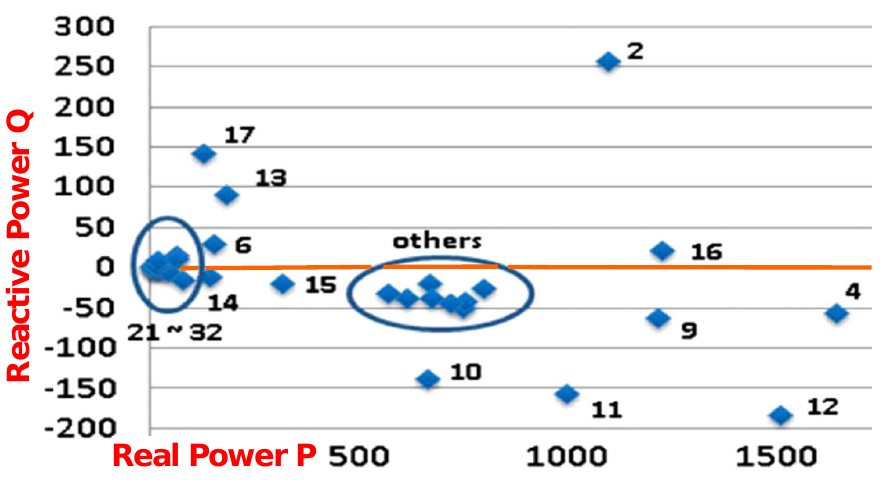
\includegraphics[width=0.70\linewidth]{real_reactive_power}
    \caption{2D-space of electrical fingerprints based on real and reactive power}
    \label{fig:real_reactive_power}
\end{figure}

\subsubsection{Voltage-Current Trajectories}
One way to create a more detailed electric fingerprint is to also consider the dimension of time.
Some appliances (for examples appliances containing motors) have very specific shapes of voltage and current curves.
This motivates using a voltage-current trajectory, see figure \ref{fig:voltage_current_trajectories}, as fingerprint.
Note that measuring these trajectories requires rather high efforts.

\begin{figure}
    \centering
    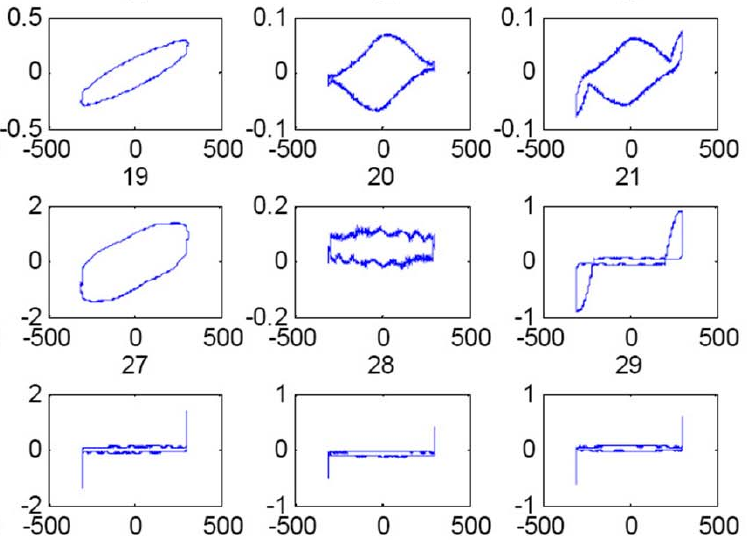
\includegraphics[width=0.60\linewidth]{voltage_current_trajectories}
    \caption{Examples of voltage-current trajectories}
    \label{fig:voltage_current_trajectories}
\end{figure}

\subsubsection{Higher Resolution Load Signatures}
If measurements are performed at $\gg 50$ Hz the shape of the current or power waveform itself can be used as a fingerprint.
Examples can be seen in \ref{fig:nilm_waveform}.
With high enough sampling frequency one can even consider the shape of single turn-on and turn-off events for different appliances.
Signatures can also be used from freqency analysis.
Another frequency-based signature is the Electromagnetic Interfernece (EMI) of different devices.
Note however that frequency measurements require very high sampling rates (As per the sampling theorem one has to sample with twice the frequency of the highest frequency component of interest).

\begin{figure}
    \centering
    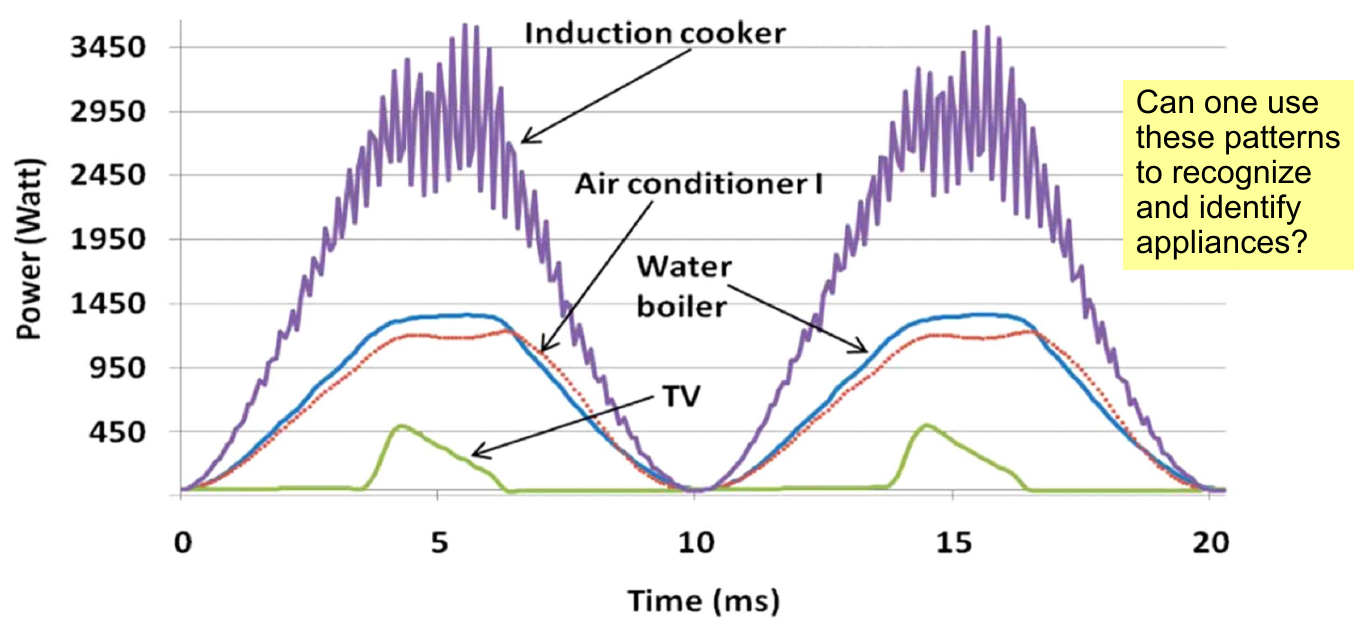
\includegraphics[width=0.70\linewidth]{nilm_waveform}
    \caption{Examples of power waveform as electric fingerprint}
    \label{fig:nilm_waveform}
\end{figure}

\subsection{Building a Signature Database}
A complete database of electric signatures can combine any of the fingerprints in \ref{sec:electric_fingerprints}.
It can include both signatures of on-off switches and of running appliances.
Building this database requires a learning phase.
Learning can be done completelty manually (recording switching on and off appliances) or by learning them automatically (supervised or unsupervised training).
Some generic features could be retrieved from global databases to simplify learning.\\

\subsection{The NILM process}
The complete NILM process generally look like

\begin{enumerate}
    \item Capture data
    \item Normalize adn filter out noise
    \item Detect events
    \item Match signature to database
    \item Application specific processing
\end{enumerate}

